\subsection{Formula di Simpson composita}

Data la proprietà di additività dell'integrale:
\begin{equation*}
	I\left(f\right) = \displaystyle\sum_{k=1}^{M} \int_{I_{k}} f\left(x\right) \:\mathrm{d}x
\end{equation*}
Si vuole approssimare l'area sottesa da $f$ nell'intervallo $I_{k}$ considerando l'area sottesa dalla parabola che interpola i punti $x_{k-1}$, $\overline{x}_{k}$ e $x_{k}$.

\highspace
Integrando tali parabole su ogni intervallo $I_{k}$, si ottiene la \definition{formula di Simpson composita}:
\begin{equation}
	I_{sim}\left(f\right) = \dfrac{H}{6} \displaystyle\sum_{k=1}^{M} \left(f\left(x_{k-1}\right) + 4f\left(\overline{x}_{k}\right) + f\left(x_{k}\right)\right)
\end{equation}
L'area sottesa alla parabole interpolante è quella tratteggiata in grigio:
\begin{figure}[!htp]
	\centering
	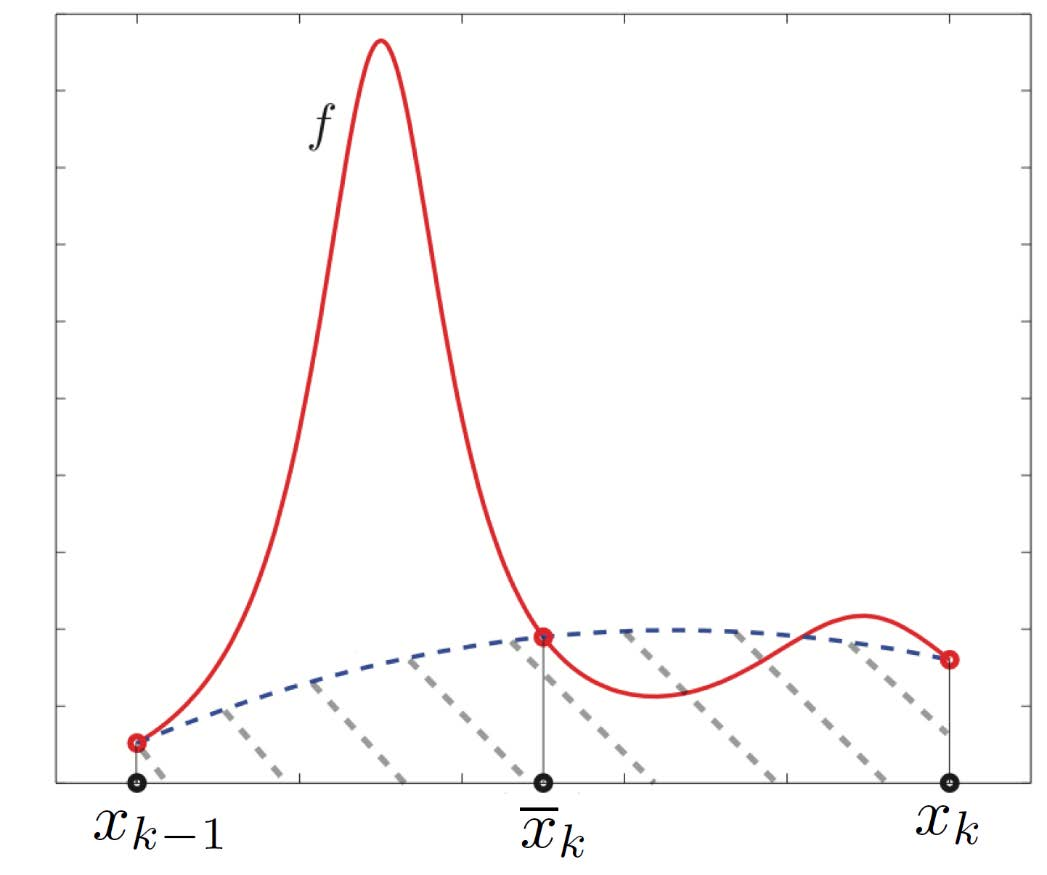
\includegraphics[width=.4\textwidth]{img/formule-di-quadratura-4.png}
\end{figure}

\noindent
Da notare che per la costruzione della forma di Simpson composita equivale all'\textbf{integrale esatto dell'interpolatore Lagrangiano composito di grado 2}:
\begin{equation}
	I_{sim}\left(f\right) = \displaystyle\int_{a}^{b} \displaystyle\prod_{2}^{H} f\left(x\right) \:\mathrm{d}x
\end{equation}
Assumendo che $f$ abbia la derivata quarta continua su $\left[a,b\right]$, allora la \definition{stima dell'errore per la formula dei trapezi composita} è:
\begin{equation}
	\left|I\left(f\right) - I_{sim}\left(f\right)\right| \le \dfrac{b-a}{2880} \underset{x}{\max} \left|f^{\left(iv\right)}\left(x\right)\right| H^{4}
\end{equation}
Si possono fare due \textbf{osservazioni} riguardo alla stima dell'errore:
\begin{enumerate}
	\item La \textbf{formula di Simpson} è di \textbf{ordine 4}.
	
	\item La \textbf{formula di Simpson} ha \textbf{grado di esattezza pari a 3}.
\end{enumerate}
Per cui, tale metodo integra i polinomi che sono globalmente di: 
\begin{itemize}
	\item Grado $r=1$ (rette)
	\item Grado $r=2$ (parabole)
	\item Grado $r=3$ (cubiche)
\end{itemize}
